\section{Aplicación en desarrollo de aplicaciones Web} 

Como aplicaciones para los casos de prueba haremos uso de 
las siguientes aplicaciones:\\
\begin{table}[h!]
    \begin{center}
      \caption{Parámetros línea comandos dependency-check}
      \label{tab:tabla 2}
      \begin{tabular}{c|c}
        \textbf{Aplicación} & \textbf{Tecnologías utilizadas}\\
        \hline
        \href{https://dvwa.co.uk/}{Damn Vulnerable Web application (dwva)} & PHP\\ 
        \href{https://github.com/bkimminich/juice-shop}{Juice Shop} & JavaScript, Angular, Node.js\\
        \href{https://github.com/WebGoat/WebGoat}{WebGoat} &  Java, Spring Boot\\
        \href{https://github.com/tobyash86/WebGoat.NET}{WebGoat.Net} & .Net Core     
      \end{tabular}
    \end{center}
  \end{table}
\newpage

\subsubsection{Damn Vulnerable Web application (DVWA)}
Siguiendo las tareas del \href{https://github.com/M0l1n3ta/PFG/blob/master/Reportes/DVWA/PPR DVWA - Plan Pruebas de Seguridad.docx}{documento de plan pruebas}
para este proyecto, realizamos las tareas que se detallan a continuación.\\

Para este proyecto no se realizará análisis de dependencias puesto que el proyecto no hace uso del componente de PHP 
necesario para realizar este tipo de análisis en proyectos PHP (\href{https://getcomposer.org/}{Composer})

La ejecución del análisis estático de código lo realizaremos a través de un
\href{https://github.com/M0l1n3ta/PFG/blob/master/Scripts/STAT/RunSonarScaner_DWVA.ps1}{script}, con el cual obtenemos 
el siguiente resultado:\\

\begin{figure}[h!]  
    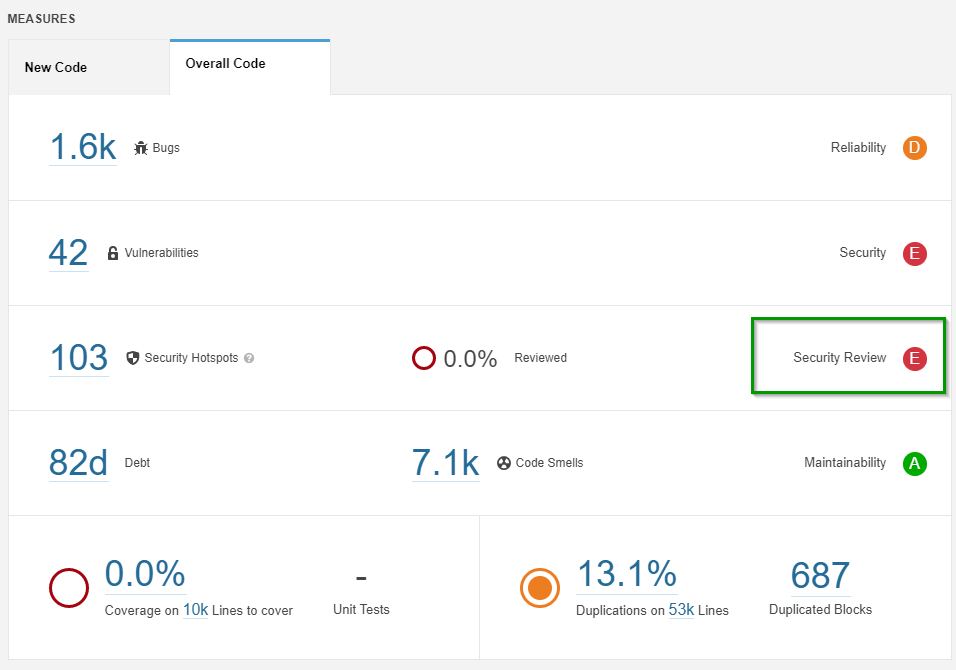
\includegraphics[width=\linewidth]{./imagenes/07_AnalisisEstatico__DVWA.png}
    \caption{Resultado análisis estatico código DVWA}  
    \label{fig:22}
\end{figure}
Como era de esperar obtiene el peor resultado posible en la medida de seguridad \textbf{“E”}
\newpage
\subsubsection{Juice Shop}
Siguiendo las tareas del documento de plan pruebas para este proyecto, realizamos las tareas que se detallan a continuación.\\

La ejecución del análisis estático de código, así como el análisis de dependencias, lo realizaremos a través de un 
\href{https://github.com/M0l1n3ta/PFG/blob/master/Scripts/STAT/RunSonarScaner_JuiceShop.ps1}{script}, con el cual obtenemos 
el siguiente resultado:\\

\begin{figure}[h!]
    \centering  
    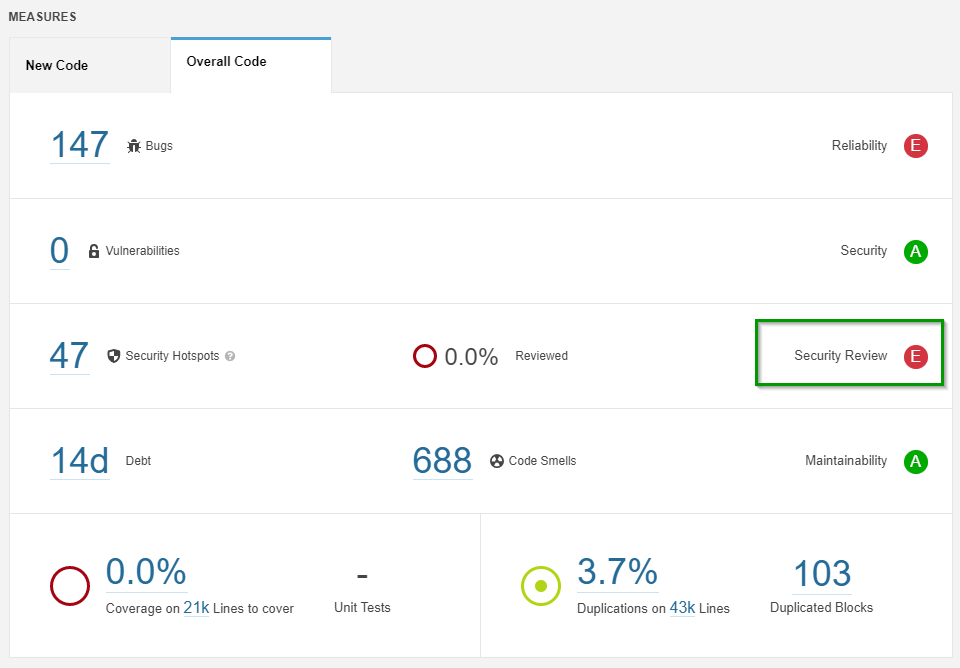
\includegraphics[width=\linewidth]{./imagenes/08_AnalisisEstatico_JuiceShop.png}
    \caption{Resultado análisis estatico código Juice Shop}  
    \label{fig:23}
\end{figure}
Como era de esperar obtiene el peor resultado posible en la medida de seguridad \textbf{“E”}
\newpage
\subsubsection{WebGoat}
Siguiendo las tareas del documento de plan pruebas para este proyecto, realizamos las tareas que se detallan a continuación.

Para ejecutar el análisis de dependencias desde Maven, debemos añadir la siguiente configuración del plugin de Dependency-Check:

\begin{listing}[h]
    \inputminted{xml}{./Ficheros/ConfiguracionPlugin_Maven.xml}
    \caption{Example from external file}
    \label{listing:4}
\end{listing}

A parte de la configuración anterior debemos añadir las siguientes propiedades:\\

\begin{listing}[h]
    \inputminted{xml}{./Ficheros/ConfigPropertiesPlugin_maven.xml}
    \caption{Example from external file}
    \label{listing:24}
\end{listing}

Para ejecutar el escáner\\

\begin{verbatim}
    mvn dependency-check:check
\end{verbatim}

La ejecución del análisis estático de código, así como el análisis de dependencias, lo realizaremos a través de un 
\href{https://github.com/M0l1n3ta/PFG/blob/master/Scripts/STAT/RunSonarScaner_WebGoat.ps1}{script}, con el cual
obtenemos el siguiente resultado:\\

\begin{figure}[h!]  
    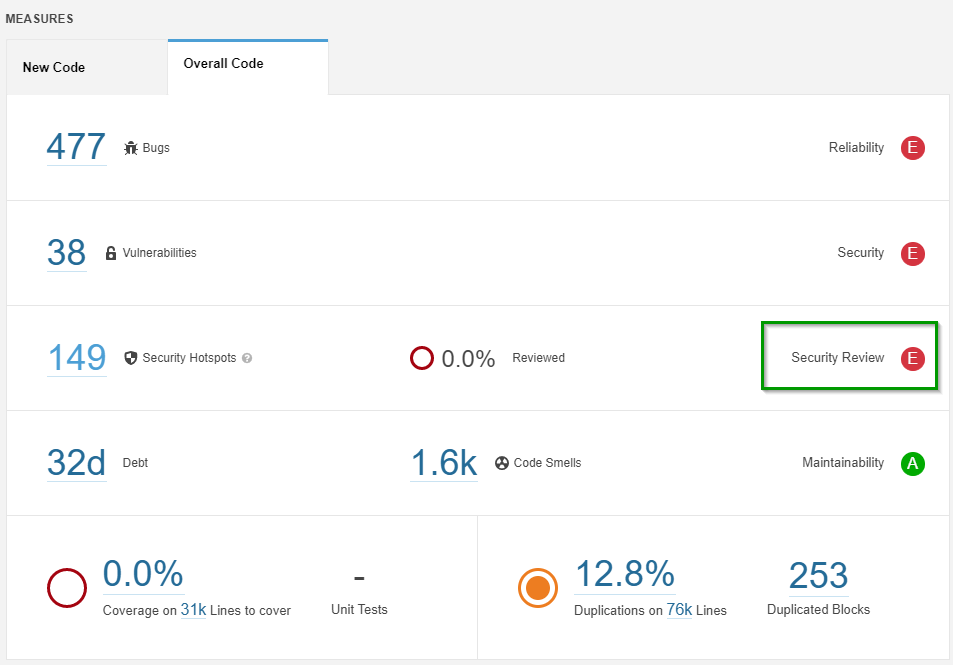
\includegraphics[width=\linewidth]{./imagenes/09_AnalisisEstatico_WebGoat.png}
    \caption{Resultado análisis estatico código WebGoat}  
    \label{fig:25}
\end{figure}

Como era de esperar obtiene el peor resultado posible en la medida de seguridad \textbf{“E”}\\

\newpage
\subsubsection{WebGoat.Net}
Siguiendo las tareas del documento de plan pruebas para este proyecto, realizamos las tareas que se detallan a continuación.

La ejecución del análisis estático de código, así como el análisis de dependencias, lo realizaremos a través de un 
\href{https://github.com/M0l1n3ta/PFG/blob/master/Scripts/STAT/RunSonarScaner_WebGoat.NET.ps1}{script}, con el cual obtenemos
el siguiente resultado:
\begin{figure}[h!]  
    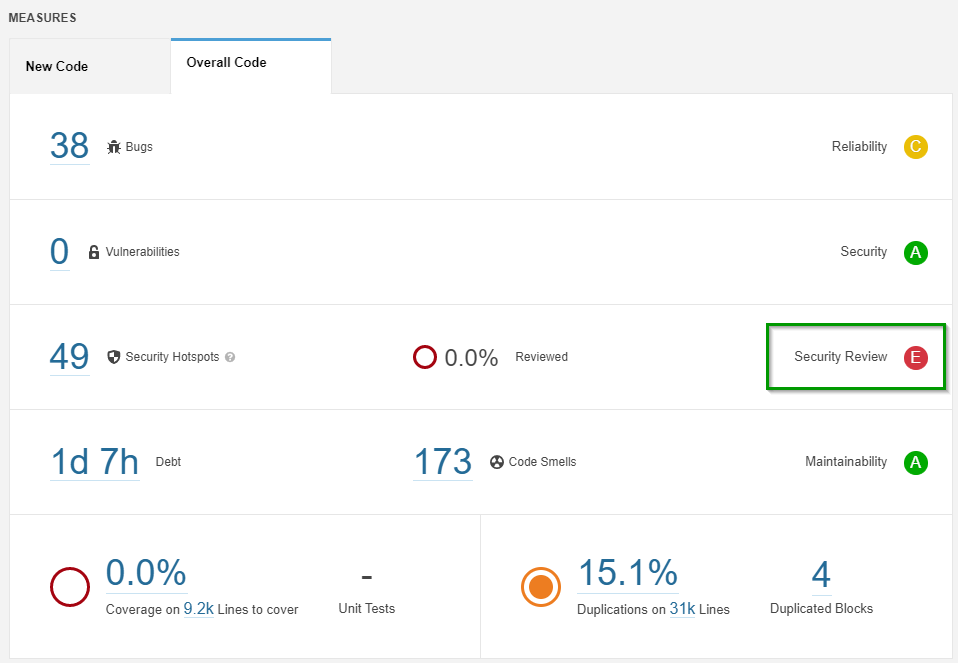
\includegraphics[width=\linewidth]{./imagenes/10_AnalisisEstatico_WebGoat.Net.png}
    \caption{Resultado análisis estatico código WebGoat}  
    \label{fig:26}
\end{figure}
Como era de esperar obtiene el peor resultado posible en la medida de seguridad \textbf{“E”}

\newpage
\section{Aplicación en desarrollo de Servicios Web} 

